
%(BEGIN_QUESTION)
% Copyright 2007, Tony R. Kuphaldt, released under the Creative Commons Attribution License (v 1.0)
% This means you may do almost anything with this work of mine, so long as you give me proper credit

Suppose a chemical reactor is heated by steam.  A temperature controller varies the amount of steam admitted to a ``jacket'' surrounding the reactor:

$$\includegraphics[width=15.5cm]{i01689x01.eps}$$

Ever since this process was placed into service, operators have complained about poor temperature control.  Several technicians have tried to tune the PID controller, but no combination of tuning constants seems to solve the problem of random reactor temperature fluctuations.  Then one day you notice that the ``random'' fluctuations of temperature are not really random at all: they directly follow fluctuations in steam supply pressure over time.

Explain the nature of the control problem (why do variations in steam supply pressure affect the reactor temperature?), and propose a solution for it.

\vskip 20pt \vbox{\hrule \hbox{\strut \vrule{} {\bf Suggestions for Socratic discussion} \vrule} \hrule}

\begin{itemize}
\item{} Like so many real-life problems, there are usually multiple solutions.  Try brainstorming more than one practical solution to this control problem!
\end{itemize}

\underbar{file i01689}
%(END_QUESTION)





%(BEGIN_ANSWER)

As the steam supply pressure rises and falls, a greater or lesser steam flow will result through the temperature valve (TV) for any given stem position.

The simplest and most direct solution to this problem is to stabilize the steam supply pressure: determine what is causing the pressure to fluctuate, and fix it!

%(END_ANSWER)





%(BEGIN_NOTES)

As the steam supply pressure rises and falls, a greater or lesser steam flow will result through the temperature valve (TV) for any given stem position.  The reactor temperature controller (TC) does not know to move the valve until a change is seen in the reactor temperature.  In other words, the controller's action is always ``after the fact.''  It does not ``know'' that it should move the valve to compensate for changed steam flow until after that different steam flow rate has altered the process temperature.

If it is not possible to stabilize the steam header pressure, another solution is to add {\it cascade} control to the system: a steam flow controller which receives a setpoint from the temperature controller.

%INDEX% Control, strategies: cascade
%INDEX% Process: steam-heated reactor vessel (generic)

%(END_NOTES)


